\cleardoublepage

\chapter{GOVERNING EQUATIONS AT GIGAHERTZ RANGE}
\label{chap:3}

\section{Specific Absorption Rate}
In general, there exists a strong correlation between heating effects and the amount of the \gls{em} power that is absorbed by human tissue.
The comprehensive measure of power absorption per unit mass is commonly expressed in terms of \gls{sar}, measured in watts per kilogram.
A seminal work by Chou~\cite{Chou1975Effects}, as referenced in~\cite{Foster2022Three}, highlights the initial appearance of the term ``\gls{sar}'' within the context of his doctoral dissertation in 1975.

\Gls{sar} serves as a quantitative measure of the rate at which \gls{em} energy is either absorbed by or dissipated in a unit mass contained within a volume element,
\begin{align}
    \label{eqn:sar_1}
    \text{SAR} = \frac{\partial}{\partial t} \left( \frac{\partial W}{\partial m} \right).
\end{align}
In cases where the exposed tissue is of constant density, $\rho$, the aforementioned relationship can be represented as
\begin{align}
    \label{eqn:sar_2}
    \text{SAR} = \frac{\partial}{\partial t} \left( \frac{\partial W}{\rho \; \partial V} \right),
\end{align}
where $V$ stands for the observed volume element.

Biological tissue is regarded as a magnetically transparent and lossy medium, characterized by a frequency-dependent relative complex dielectric permittivity, $\varepsilon^*$, and relative permeability, $\mu_r = 1$~\cite{Sasaki2014Measurement}.
Consequently, under practical circumstances, \gls{sar} can be assessed by using the following expression:
\begin{align}
    \label{eqn:sar_3}
    \text{SAR} = \frac{\sigma \; \left| \mathbf{E} \right|^2}{2 \rho}.
\end{align}
Here, $\sigma$ represents the conductivity of the tissue measured in siemens per meter, while $\mathbf{E}$ is the peak value of the electric field at a specific point within tissue.

In cases of brief exposure with negligible heat loss, the temperature rise can be approximated as
\begin{align}
    \label{eqn:sar_4}
    \text{SAR} = C \; \frac{\partial T}{\partial t},
\end{align}
where $C$ represents specific heat capacity $\left[ \SI{}{\joule\per\kg\per\celsius} \right]$, and $T$ denotes the temperature measured in degrees Celsius.
However, in realistic exposure scenarios that cannot be approximated by using homogeneous models, heat loss becomes significant due to the rapid diffusion caused by active thermoregulatory mechanisms.
Consequently, when \gls{sar} is used as a surrogate for temperature rise, it is necessary to spatially average it either over the whole body or, in the case of local exposure, over the volume of tissue weighing \SI{10}{\g}~\cite{McIntosh2011SAR}.

The volume-averaged \gls{sar} over \SI{10}{\g},
\begin{align}
    \text{10-g SAR} = \frac{1}{2} \; \int_{V_\text{10 g}} \frac{\sigma \; \left |\mathbf{E} \right|^2}{\rho} \; \mathrm{d}V,
\end{align}
has been shown to correlate with temperature rise well up to \SI{6}{\GHz}, regardless of whether a homogeneous cubical or a morphologically accurate body model is employed~\cite{Hirata2009correlation}.
In scenarios where simplistic tissue models are utilized, the peak-spatial \gls{sar} can also serve as an indicator of temperature rise, particularly in the frequency bands of \SIlist{150;400;900}{\MHz}.
This observation is supported by investigations employing a realistic \gls{3-d} human body model~\cite{Hirata2006Correlation}.
At higher frequencies, particularly above \SI{6}{\GHz}, the correlation between peak-spatial \gls{sar} and maximum temperature rise is only modest for realistic exposure scenarios involving morphologically accurate body models~\cite{Morimoto2016Relationship}.

In the context of whole-body exposure, assessment of the whole-body averaged \gls{sar} is contingent upon factors such as the spatial distribution of the internal electric field, electric conductivity of tissue, and tissue density.
Thus, the whole-body averaged \gls{sar} can be defined as the ratio of the total power absorbed in the whole body and the whole body mass:
\begin{align}
    \label{eqn:sar_wb}
    \text{whole-body SAR} = \frac{1}{2} \; \int_{V_\text{wb}}\frac{\sigma \; \left |\mathbf{E} \right|^2}{\rho} \; \mathrm{d}V,
\end{align}

Several numerical analyses have been conducted to investigate various averaging schemes in terms of their efficacy in predicting local temperature rise~\cite{Hirata2009correlation,McIntosh2011SAR}.
Consensus has been reached regarding the suitability of a cubic averaging mass of \SI{10}{\g} as an appropriate equivalent volume for spatial averaging up to \SI{6}{\GHz}, regardless of the tissue type.
It is worth emphasizing that a 10-g volume corresponds approximately to \SI{2.15}{\cm\cubed} cube, assuming that the density of exposed tissue is the same as that of water, i.e., \SI{1000}{\kg\per\m\cubed}.

On average, the time required to reach a steady state for the case of the whole body exposure is \SI{30}{\minute} minimum.
Conversely, for localized exposure, duration of \SI{6}{\minute} is deemed sufficient.
The consideration of temporal averaging for whole-body exposure is based on both analytical approximations provided in the \gls{icnirp} guidelines~\cite{ICNIRP2020Guidelines} and empirical studies~\cite{Hirata2008FDTD,Nelson2013High}.
The time constant is governed by the rate of heat exchange between the core of the body and the surrounding environment~\cite{Adair2003Thermoregulatory}.
The temporal averaging for localized exposure is more intricate as it depends on two distinct factors, such as the rate of convective heat exchange by blood flow and conduction of heat from the exposed area~\cite{Foster2017Thermal}.
Simple analytical models~\cite{Foster2017Thermal} and a detailed numerical analysis~\cite{Morimoto2017Time} indicate that the overall dissipation of heat from an exposed region is primarily governed by thermal convection through blood flow.
In turn, thermal convection depends on multiple factors, but is generally accepted that after \SI{6}{\minute}, a steady state is reached in most exposure scenarios.

\section{Transition to Area-Averaged Dosimetric Quantities}
In 1998 version of the \gls{icnirp} guidelines~\cite{ICNIRP1998Guidlines}, \gls{sar} was used up to \SI{10}{\GHz}, whereas the power density was used above this transition frequency.
However, in 2005 version of the \gls{ieee} standard~\cite{IEEE2005Standard}, the transition frequency was adjusted to \SI{3}{\GHz}.
This discrepancy resulted in a discontinuity in the exposure limits at the transition frequency~\cite{Colombi2015Implications}.
Recent studies demonstrated that \gls{sar} no longer serves as an appropriate surrogate for predicting local temperature rise above \SI{6}{\GHz}, particularly at \gls{mmw}.
This is primarily due to the fact that at such high frequencies, \gls{em} energy is deposited predominantly in cutaneous tissue~\cite{Ziskin2018Tissue,Zhadobov2011Millimeter}.
With an increase in frequency, the \gls{emf} penetration depth decreases, resulting in a more superficial distribution of \gls{em} energy.
Therefore, the power density absorbed in the skin provides a better estimation of the maximum temperature rise on the surface of the exposed body at the \SIrange{6}{300}{\GHz} range~\cite{Funahashi2018Area-averaged}.

The need for the harmonization between the volume-averaged \gls{sar} and area-averaged power density and determination of a break-point between exposure limits was recognized as early as 2011~\cite{McIntosh2011SAR}.
In this study, authors argue that the combined results of simple planar and complex body modeling did not offer a clear indication of which metric exhibited a stronger correlation with the induced temperature rise from \gls{rf} heating at the \SIrange{3}{10}{\GHz} range.
However, from a practical standpoint, \SI{6}{\GHz} was identified as the transition frequency due to the ease of assessing spatially averaged power density by comparison to volume-averaged \gls{sar}.

Based more recent analytical~\cite{Foster2016Thermal,Foster2017Thermal,Ziskin2018Tissue} and numerical studies~\cite{Hirata2019Setting}, the transition frequency has been set to \SI{6}{\GHz} in the recent updates of the \gls{icnirp} guidelines and \gls{ieee} standard, leading to the long-awaited harmonization.

\subsection{Absorbed/Epithelial Power Density}
Dissipation of power density within the tissue exhibits an exponential decline from the surface towards deeper regions.
Thus, the spatially averaged \gls{apd} on the surface is defined as
\begin{align}
    \label{eqn:apd}
    S_\text{ab} = S(z=0) \; \int_{z=0}^{z_\text{max}} e^{ -\nicefrac{2z}{\delta}} \; \mathrm{d}z,
\end{align}
where $S(z=0)$ represents the specific \gls{apd} averaged on the exposed surface, $\delta$ stands for the perpendicular penetration depth into the tissue (along the $z$-axis in this context), whereas $z_\text{max}$ denotes the depth of the exposed tissue which must be sufficiently large to compensate for $\delta$.

The specific \gls{apd} at $z=0$, averaged over area $A$ is expressed as
\begin{align}
    \label{eqn:specific_apd}
    S(z=0) = \frac{1}{A} \; \iint_A \rho(x, y, 0) \; \text{SAR}(x, y, 0) \; \mathrm{d}x \mathrm{d}y.
\end{align}

To illustrate the exponential decay, let's consider the following example.
Firstly, \num{1000} values are sampled from a continuous uniform distribution constrained within the range from \SI{0}{\watt\per\m\squared} and the maximum permissible \gls{ipd} at \SIlist{10;30;60;100}{\GHz}.
The mean and standard deviation of these sampled values are calculated.
Next, we estimate the specific area-averaged \gls{apd} using the following expression:
\begin{align}
    \label{eqn:specific_apd_approx}
    S(z=0) = T \cdot \text{IPD}.
\end{align}
Here, $T$ denotes the transmission coefficient, which is defined as
\begin{align}
    \label{eqn:transmittance}
    T = 1 - \left| \Gamma \right|^2.
\end{align}
The reflection coefficient,  $\Gamma$, is derived from the dielectric properties of the tissue, shape of the body surface, incident angle and polarization.
For this purpose, we consider a scenario involving a plane wave with normal incidence onto a planar, dry skin half-space.
The dielectric properties are characterized by the relative complex permittivity~\cite{Wu2015human},
\begin{align}
    \label{eqn:rel_complex_permittivity}
    \varepsilon^* = \varepsilon' + j \; \varepsilon'',
\end{align}
where
\begin{align}
    \varepsilon'' = \frac{\sigma}{2 \pi f \varepsilon_0}.
\end{align}
The value of $\varepsilon'$ is extracted from~\cite{Gabriel1996Compilation} at the corresponding frequency. 
This sampling procedure is repeated \num{1000} times to acquire the expected specific \gls{apd} within the range of values that can are approximated from the range of \gls{ipd}s.
Finally, in~\cref{fig:power_density_absorption}, the intensity of the power density at $z=\SI{0}{\mm}$ is depicted with a solid line, whereas the value of the power density absorbed at a depth of \SI{1}{\mm} into the dry skin is represented by a dashed line.
\begin{figure}[ht]
    \centering
    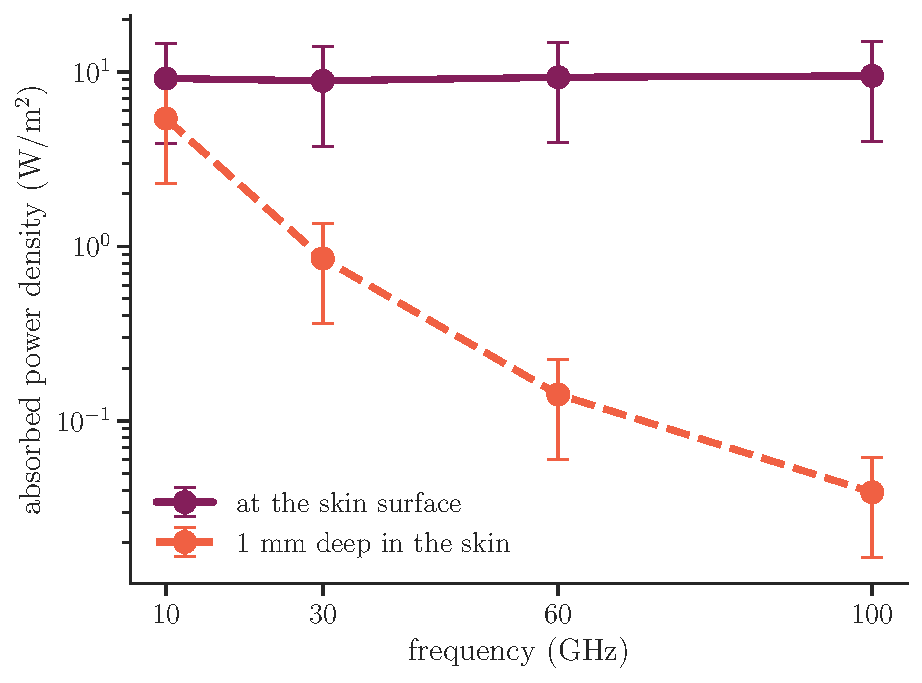
\includegraphics[width=0.8\textwidth]{artwork/power_density_absorption.pdf}
    \caption{Power density as a function of frequency at the skin surface (solid line) and at \SI{1}{\mm} depth in homogeneous dry skin (dashed line).}
    \label{fig:power_density_absorption}
\end{figure}
With an increase in frequency, and for \gls{ipd} bounded between \SI{0}{\watt\per\m\squared} and the maximum allowable value~\cite{ICNIRP2020Guidelines,IEEE2019Standard}, the power density at the surface remains relatively constant at approximately \SI{9}{\watt\per\m\squared}.
However, even at a depth of \SI{1}{\mm} perpendicular into the skin, $S_\text{ab}$ drops respectively by \SIlist{40.98;90.39;98.48;99.59}{\percent} at \SIlist{10;30;60;100}{\GHz} by using the corresponding surface value as a reference.

In the updated version of the \gls{icnirp} guidelines~\cite{ICNIRP2020Guidelines} and \gls{ieee} standard~\cite{IEEE2019Standard}, two definitions of the spatially averaged \gls{apd} have been adopted, both stemming from the Poynting theorem.
The first definition of is given in terms of \gls{tpd}~\cite{Funahashi2018Area-averaged}
\begin{align}
    \label{eqn:tpd}
    \text{TPD}(x, y) = \int_{z = 0}^{z_\text{max}} \rho(x, y, z) \; \text{SAR}(x, y, z) \; \mathrm{d}z,
\end{align}
spatially averaged across the exposed surface of tissue, $A$
\begin{align}
    \label{eqn:apd_1}
    S_\text{ab, v} = \frac{1}{A} \iint_{A} \text{TPD}(x, y) \; \mathrm{d}A.
\end{align}
The tissue surface is positioned at $z = 0$, whereas $z_\text{max}$ should be sufficiently greater than the penetration depth.
The second formula is given as the spatially averaged power density flux on the exposed surface
\begin{equation}
    \label{eqn:apd_2} 
    S_\text{ab, s} = \frac{1}{2A} \iint_{A} \Re \big[\mathbf{E}(x, y) \times \mathbf{H}^*(x, y) \big] \; \mathbf{\hat n} \; \mathrm{d}A
\end{equation}
where $\mathbf{E}$ and $\mathbf{H}$ are peak values of the complex phasor electric and magnetic field on the surface, respectively, $\Re$ denotes the real part of the vector field, and the asterisk represents the complex conjugate operator.
Integral variable vector, $\mathbf{\hat n} \; \mathrm{d}A$, is set perpendicularly to the exposed surface, where  $\mathbf{\hat n}$ corresponds to the unit normal vector to the surface.

It is outlined in~\cite{Hashimoto2017averaging} that a square \SI{4}{\cm\squared} evaluation surface provides a close approximation to maximum temperature rise due to \gls{rf} heating above \SI{6}{\GHz}.
The results are based on the heating factor, the ratio between the spatially averaged \gls{apd} and maximum temperature rise, computed on a a multiple-layer tissue model exposed to three different sources of \gls{emf}s: the plane wave, a dipole antenna, and an antenna array.
The schematic of the exposed tissue is shown in~\cref{fig:averaging_surface}.
\begin{figure}[t]
    \centering
    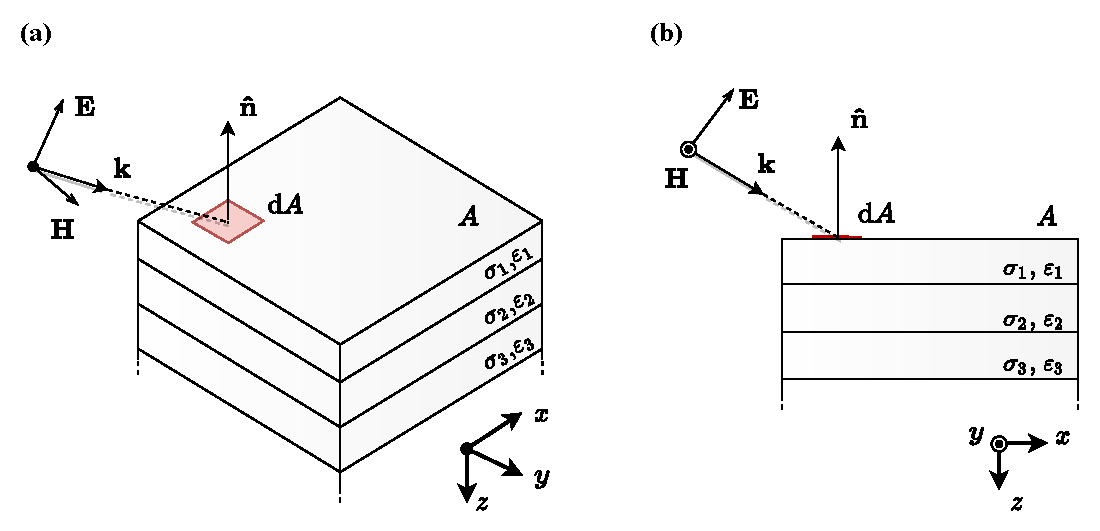
\includegraphics[width=\textwidth]{artwork/averaging_surface.pdf}
    \caption{Evaluation surface on a multiple-layer tissue-equivalent block model: (a) isometric projection, (b) orthographic projection.}
    \label{fig:averaging_surface}
\end{figure}
The area of \SI{4}{\cm\squared} achieves consistency with the volume-averaged dosimetric quantities below \SI{6}{\GHz} as the front facing surface of 10-g cubic volume is approximately of the same area ($2.15 \times 2.15$ \SI{}{\cm\squared} assuming constant tissue density of \SI{1000}{\kg\per\m\cubed}).
\begin{figure}[t]
    \centering
    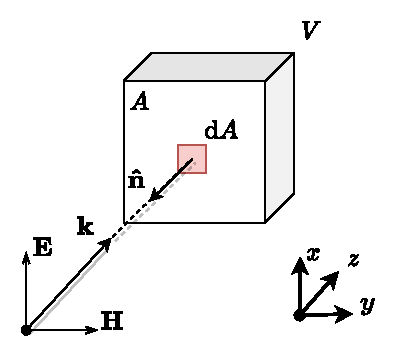
\includegraphics[width=0.42\textwidth]{artwork/averaging_volume.pdf}
    \caption{A 10-g cubic volume for assessment of local exposure to radio-frequency electromagnetic fields below \SI{6}{\GHz}.}
    \label{fig:averaging_volume}
\end{figure}

At frequencies above \SI{30}{\GHz}, the area of \SI{4}{\cm\squared} is not suitable for spatial averaging because of the possibility of inhomogeneous field distribution.
Therefore, \gls{apd} should be averaged on square \SI{1}{\cm\squared} evaluation plane to capture the focused beams.

\subsection{Equivalence of Absorbed/Epithelial Power Density Definitions}
In~\cref{eqn:apd_2}, the cross product between peak values of the complex phasor electric and magnetic field represents the power density vector field whose direction is perpendicular to the incident surface.
Essentially, this cross product represents the Poynting vector, given in~\cref{eqn:poynting-vector}.

The surface integral of the normal component of the time-averaged Poynting vector on the exposed surface results in a scalar value, which corresponds to the overall flux passing through that surface.
The divergence theorem, commonly referred to as the Gauss-Ostrogradsky theorem, establishes a relationship between the flux of a vector field through a closed surface and the divergence of a field within an enclosed volume.
In other words, it states that the surface integral of a vector field across a closed surface is equivalent to the volume integral of the divergence within the region enclosed by that surface.

Given the aforementioned principles, it can be deduced from the Poynting theorem, given in~\cref{eqn:poynting-theorem}, that the definitions of the spatially averaged \gls{apd} are equivalent if the surface surrounding a particular volume of tissue is closed and that there are no active sources within this volume.

In both definitions, it is assumed that the Poynting vector is averaged in time and is given in its corresponding phasor notation.
However, the Poynting vector in the time-harmonic variation is written as
\begin{align}
    \label{eqn:poynting-vec-time-harmonic}
    \mathcal{P} &= \mathcal{E} \times \mathcal{H} \notag\\
                &= \Re \left( \mathbf{E} \; e^{j \omega t} \right) \times \Re \left( \mathbf{H} \; e^{j \omega t} \right) \notag\\
                &= \frac{1}{2} \; \left( \mathbf{E} \; e^{j \omega t} + \mathbf{E}^*  \; e^{-j \omega t} \right) \times \frac{1}{2} \; \left( \mathbf{H} \; e^{j \omega t} + \mathbf{H}^*  \; e^{-j \omega t} \right) \notag\\
                &= \frac{1}{2} \; \Re \left( \mathbf{E} \times \mathbf{H}^* \right) + \frac{1}{2} \; \Re \left( \mathbf{E} \times \mathbf{H} \; e^{2j \omega t} \right), 
\end{align}
where $t$ is the time domain, and the normalization factor $\nicefrac{1}{2}$ appears as \gls{emf} components are given by their corresponding peak values.
From \cref{eqn:poynting-vec-time-harmonic}, the time-averaged Poynting vector is then written as
\begin{align}
    \label{eqn:poynting-vec-time-avg}
    \mathbf{P} = \frac{1}{2} \; \Re \left( \mathbf{E} \times \mathbf{H}^* \right).
\end{align}

The time-averaged total power crossing a \gls{2-d} surface in \gls{3-d} space can then be written as
\begin{align}
    \label{eqn:poynting-flow}
    P_\text{tot} &= \oint_S \mathbf{P} \; \mathrm{d}\mathbf{S} \notag\\
                 &= \frac{1}{2} \; \oint_S \Re \big( \mathbf{E} \times \mathbf{H}^* \big) \; \mathbf{\hat n} \; \mathrm{d}S.
\end{align}
Once the total power is spatially averaged on the exposed surface, $\nicefrac{P_\text{tot}}{A}$, the resulting quantity is equivalent to a radiated power density uniformly distributed over the averaging area $A$ and crossing this surface.

Now, by enforcing the divergence theorem onto the Poynting flow given in \cref{eqn:poynting-flow} through any closed surface, $S$, bounding an arbitrary volume, $V$, under the assumption that there are no active sources inside that volume, the above expression can be rewritten as
\begin{align}
    P_\text{tot} &= \frac{1}{2} \; \iiint_V \nabla \left [ \Re \left( \mathbf{E} \times \mathbf{H}^* \right) \right] \; \mathrm{d}V \notag\\
                 &= -\frac{1}{2} \; \iiint_V \sigma \; |\mathbf{E}|^2 \; \mathrm{d}V.
\end{align}
By separating the total power loss in the expression above into the surface integration of the line integral and, subsequently, averaging it spatially across the surface facing the direction of the impinging \gls{em} wave as
\begin{align}
    \frac{P_\text{tot}}{A}  &= \frac{1}{2A} \iiint_V \sigma \; |\mathbf{E}|^2 \; \mathrm{d}V \notag\\
                            &= \frac{1}{2} \; \iint_A \int_z \sigma \; |\mathbf{E}|^2 \; \mathrm{dA} \mathrm{d}z,
\end{align}
the above expression matches the definition of the spatially averaged \gls{apd} given in~\cref{eqn:apd_1}.

Finally, it is clear that the definitions are equivalent if the averaging surface for $S_\text{ab, s}$ is closed and free of sources.
This condition must be met to account for the power deposited within the volume of interest.
This means that $S_\text{ab, s}$, given as the surface integral of the vector field in~\cref{eqn:apd_2}, should take into account the entire closed surface surrounding the exposed volume and not only on the directly exposed, i.e., the front surface facing only the direction of the impinging \gls{em} wave (\cref{fig:averaging_volume}).
As this is not the case, it should be expected that $S_\text{ab, v}$ will always yield values greater than $S_\text{ab, s}$.
However, above \SI{6}{\GHz}, the power penetration depth is at most about \SI{8}{\mm}, which makes this difference only marginal.
Therefore, it may be disregarded in practice as the overall contribution of the absorption in deeper tissues is less then \SI{10}{\percent}~\cite{Li2023Calculated}.

\section{Incident Power Density}
\gls{ipd} serves as the \gls{rl} in the \gls{icnirp} guidelines~\cite{ICNIRP2020Guidelines} and the \gls{erl} in the \gls{ieee} standard~\cite{IEEE2019Standard}.
It is defined as the magnitude of the time-averaged Poynting vector, as expressed in the following equation:
\begin{align}
    \label{eqn:ipd}
    S_\text{inc} = \left| \mathbf{E} \times \mathbf{H}^* \right|.
\end{align}
For far-field exposure, \gls{ipd} can be simplified to the following expression:
\begin{align}
    \label{eqn:ipd-far-field}
    S_\text{inc} = \frac{\left| \mathbf{E} \right|^2}{Z_0} = \left| \mathbf{H} \right|^2 \; Z_0.
\end{align}
where $Z_0$ represents the characteristic impedance of free space.
Herein, the field components are treated as \gls{rms} values.

The approximation in~\cref{eqn:ipd-far-field} is a valid if the conditions of the far field are met.
This generally applies during the assessment of whole-body exposure or local exposure above \SI{6}{\GHz}, provided that the separation distance from the antenna is greater than $\nicefrac{\lambda}{2 \pi}$, where $\lambda$ denotes the wavelength of the incident field.
This distance effectively predicts the margin between the reactive and radiative near field~\cite{Carrasco2019Exposure}.
The plane-wave reflection coefficient, $\Gamma$, can be employed to establish a correlation between the incident and absorbed \gls{emf}s in the far field
\begin{align}
    \label{eqn:ipd-corr}
    S_\text{inc} = \frac{S_\text{ab}}{1 - \left| \Gamma \right|^2}.
\end{align}
However, further considerations are required for the near field.

In the far field, the Poynting vector is entirely real, and the direction of the flux remains constant over time.
On the other hand, in the near field of an antenna, this is no longer the case as reactive components of the field may contribute to the overall absorption of energy in the exposed body~\cite{Kuster1992Energy}.
Consequently, all components of the Poynting vector should be considered which makes the correlation-based formula outlined in \cref{eqn:ipd-corr} no longer accurate.

Both the \gls{icnirp} guidelines~\cite{ICNIRP2020Guidelines} and \gls{ieee} standard~\cite{IEEE2019Standard} state that the \gls{rl}s cannot be used to determine compliance in the reactive near field and \gls{br}s should be assessed instead.
Nevertheless, in the recent \gls{ieee} Guide for the definition of the \gls{ipd} to correlate surface temperature rise~\cite{IEEE2021Guide}, two distinct definitions of the \gls{ipd} have been analyzed even in the near field.

The first one is the surface-normal propagation-direction power density into the evaluation surface,
\begin{align}
    \label{eqn:ipd-normal}
    S_\text{inc, n} = \frac{1}{2 A} \; \iint_A \Re \left( \mathbf{E} \times \mathbf{H}^* \right) \; \mathbf{\hat n} \; \mathrm{d}A.
\end{align}
Here $\mathbf{E}$ and $\mathbf{H}$ represents the peak values of the complex phasor electric and magnetic field in free space, respectively.

The second definition takes into account the total propagating power density into the evaluation surface,
\begin{align}
    \label{eqn:ipd-magnitude}
    S_\text{inc, tot} = \frac{1}{2A} \iint_A \left | \Re \left( \mathbf{E} \times \mathbf{H}^* \right) \right| \; \mathrm{d}A.
\end{align}

Both definitions imply spatial averaging over the evaluation surface of area $A$.
The evaluation surface is defined as a square projection of the exposed region of tissue, where, unlike in the case of the spatially averaged \gls{apd}, incident components of the complex phasor electric and magnetic field are considered (\cref{fig:averaging_surface_fs}).
\begin{figure}[t]
    \centering
    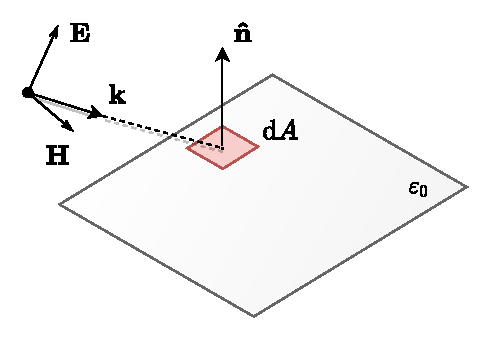
\includegraphics[width=0.46\textwidth]{artwork/averaging_surface.fs.pdf}
    \caption{Evaluation surface in free space for the averaging of the incident power density.}
    \label{fig:averaging_surface_fs}
\end{figure}

When the power density is assessed in the near field of a radiating source, the tangential components of the Poynting vector are not negligible compared to its surface-normal components.
The definition of the spatially averaged \gls{ipd} via its norm is shown to be slightly better correlated with maximum temperature rise.
However, this has been tested only considering several exposure scenarios in~\cite{IEEE2021Guide} and the overall analysis has shown that the observed difference is marginal and can mainly be attributed to near-field conditions as both definitions correlate well with temperature rise (Pearson's $r$ above 0.7).

\section{State of Research}
Choosing an appropriate spatial averaging technique is crucial for computing power density distribution on the surface on the exposed tissue.
The \gls{fdtd} method~\cite{Sullivan1987Use} is the standard numerical method of choice in numerical dosimetry for \gls{rf}-\gls{emf} simulations, owing to the advent of polished commercial software~\cite{Hirata2021Human}.
However, accurate power density values at \gls{5g} frequencies, including \gls{mmw}, on conformal surfaces of nonplanar body parts require structural rather than the grid-like spatial domain discretization~\cite{Poljak2018conformal}.
In regular grid cases, the surface is implicitly reconstructed using cubical cells, approximating spatial averaging as the sum of cell contributions.
In structural mesh cases, the surface is reconstructed using \gls{2-d} simplices and efficient quadrature schemes~\cite{Dunavant1985High,Dunavant1985Economical}.

The approach presented in this thesis does not require any priors related to positional relationship of points considering which the power density is to be spatially averaged.
Rather, it takes unorganized point set (points sampled on the nonplanar evaluation surface) as an input and estimates the unit normal in each point together with the size of the overall conformal averaging area.
From here, the spatial averaging is performed by approximating surface integrals in \gls{2-d} projected space (either by using close-form analytical formulas for the cylinder and sphere or by using the \gls{pca} for anatomical models).
More details are available in subsequent chapters.

The current state of research is reviewed based upon the available studies accessible through the EMF-portal platform.
The EMF-portal effectively summarizes scientific research data on various effects of \gls{emf}s on the human body.
The core of the EMF-portal is the literature database with \num{38786} publications and \num{7002} summaries of individual scientific studies\footnote{The total number of papers in the database was read on 2023, May 30th at: \url{https://www.emf-portal.org/en}}.

The following query was used to extract relevant studies:
\begin{verbatim}
    (power OR "power density")
    AND (average OR averaged OR area OR spatially)
    AND year=x
    AND (topic=technical_dosimetric
         OR topic=law_recommendation_guideline
         OR topic=review_survey_summary)
    AND (frequencyRange=radio_frequency
         OR frequencyRange=mobile_communications)
\end{verbatim}
where keywords are either ``power'' or ``power density'' together with either ``average'', ``averaged'', ``area'' or ``spatially''.
Keywords such as ``incident'', ``transmitted'', ``absorbed'' or even ``epithelial'' have been deliberately omitted in order to include both exposure assessment and computational dosimetry studies in the consideration regardless of authors' preference of terminology.
Additionally, the selected topics include technical dosimetry studies, laws, recommendation documents or guidelines associated with the aforementioned keywords, and review studies.
Finally, the selected frequency range includes all bands that are classified within \gls{rf} and mobile communications (above \SI{10}{\MHz}).

The purpose here is to review only the studies related to spatial averaging of power densities on the surface of the exposed tissue above \SI{6}{\GHz}.
Thus, the studies which refer to the \SIrange{6}{300}{\GHz} range are manually extracted, taking into account the publication year of each research paper from 1998 (the year of the previous version of the \gls{icnirp} guidelines~\cite{ICNIRP1998Guidlines}) to 2023 (the year of writing the thesis).
A special emphasis is on the most recent studies, written after 2019/2020, which coincide with the introduction of the spatially averaged \gls{apd} as the \gls{br} for limiting local exposure to \gls{emf}s at the \SIrange{6}{300}{\GHz} range.

In the 1998 edition of the \gls{icnirp} guidelines~\cite{ICNIRP1998Guidlines}, exposure limits \SI{10}{\GHz} were established based on the spatially averaged \gls{ipd} on a projected square-shape \SI{20}{\cm\squared} area.
Unrestricted and restricted (occupational) exposure corresponded to values of \SIlist{10;50}{\watt\per\meter\squared}, respectively.
Furthermore, local exposure was quantified by spatially averaging \gls{ipd} on the projected square-shape \SI{1}{\cm\squared} area, with limits of \SIlist{200;1000}{\watt\per\meter\squared} for unrestricted and restricted (occupational) exposure, respectively.

Contrary, the 1999 edition of the \gls{ieee} standard~\cite{IEEE1999Standard} defined maximum permissible exposure in terms of either the \gls{rms} electric and magnetic field strength, equivalent plane-wave power densities, and induced currents within the human body.
Above \SI{6}{\GHz}, restrictions for local exposure of specific body parts were determined by using the spatially averaged \gls{ipd}.
The limit for restricted exposure was set to \SI{100}{\watt\per\meter\squared}, whereas for unrestricted exposure, it varied with frequency up to \SI{15}{\GHz} and was fixed at \SI{100}{\watt\per\meter\squared} above \SI{15}{\GHz}.
These values were derived upon the steady-state volume-averaged \gls{sar}, with spatial averaging achieved by computing the \gls{rms} value of \gls{ipd} over an area equivalent to the vertical cross section of the human body at a minimum distance of \SI{20}{\cm\squared} from any object.

The 2005 edition of the \gls{ieee} standard~\cite{IEEE2005Standard} established an exposure limit in terms of the spatially averaged \gls{ipd} of \SI{10}{\watt\per\meter\squared} for unrestricted exposure at \SIrange{3}{10}{\GHz} range.
The power density should be spatially averaged over a contiguous area corresponding to $100 \cdot \lambda^2$, where $\lambda$ represents the wavelength of the incident \gls{emf}.
Moreover, within the \SIrange{3}{30}{\GHz} range, the peak-spatial \gls{ipd} was defined as $18.56 \cdot f_G^{0.699}$, whereas above above \SI{30}{\GHz}, it was set to \SI{200}{\watt\per\m\squared}.
Here, $f_G$ denotes the frequency of the \gls{emf}s in gigahertz.
The specific details regarding the averaging area and spatial sampling procedure for power density were not explicitly specified in the latter case.


\Cref{tab:summary_1998_2018} provides a concise overview of studies published between 1998 and 2017 that address the averaging of power densities, with most of these studies adopting the spatial averaging techniques outlined in~\cite{ICNIRP1998Guidlines}, with some exceptions of note.
\begin{sidewaystable}[ht]
\begin{center}
\caption{Summary of the studies published between 1998 and 2017 related to spatially averaged power densities.}
\label{tab:summary_1998_2018}
\begin{tabularx}{\textwidth}{|X|X|X|X|X|}
\hline
\textbf{Study} & \textbf{Scope} & \textbf{Exposure scenario} & \textbf{Methods} & \textbf{Averaging scheme} \\
\hline
Hirata et al. (2000)~\cite{Hirata2000Temperature} & investigation of a temperature hot-spot formation in the human eye and its dependence on \gls{sar} and additional variables & human eye voxel model exposed to plane wave (\SI{50}{\watt\per\meter\squared}) at \SIrange{0.6}{6}{\GHz} & \gls{fdtd} with the maximum cell size of $\nicefrac{\lambda}{10}$; $\lambda$ is the shortest wavelength in considered exposure scenarios & \gls{rms} of \gls{ipd} on surface approximately equivalent to the vertical cross-section (projected area) of the eye with a volume of \SI{9.9}{\cm\cubed} \\
\hline
Walters et al. (2000)~\cite{Walters2000Heating} & conduction of measurements for thermal pain thresholds; development of the \gls{1-d} thermal model & a human subject's back briefly exposed to \gls{rf} \gls{emf}s (\SI{18}{\kW\per\meter\squared}) at \SI{94}{\GHz} at the distance of \SI{188}{\cm} & readings at \SI{5}{\mm} increments over the evaluation plane which corresponds to a projection of a subject's back & mean value of the power density within the most exposed region (i.e., where \SI{90}{\percent} of the total power density is distributed) \\
\hline
Faraone et al. (2000)~\cite{Faraone2000Estimation} & estimation of the spatially averaged \gls{ipd} in the vicinity of cellular base-station antennas & free space field evaluation based on the dipole and collinear array antenna at different separation distances & analytical formulations & analytical formulations that estimate a single-point worst case measure\\
\hline
Anderson et al. (2010)~\cite{Anderson2010SAR}, McIntosh and Anderson (2010)~\cite{McIntosh2010SAR} & definition of the appropriate exposure metric at the \SIrange{1}{10}{\GHz} range and the transition frequency from \gls{sar} to \gls{ipd} & simple multiple-layer block and realistic human head voxel models exposed to a plane wave and dipole antennas at \SI{10}{\mm} separation distance & \gls{fdtd} with the maximum cell size of $\nicefrac{\lambda}{10}$; $\lambda$ is the shortest wavelength in considered exposure scenarios & peak value of \gls{ipd} for the block model; \gls{rms} of \gls{ipd} averaged on a square \SI{20}{\cm\squared} projection for head models\\
\hline
Colombi et al. (2015)~\cite{Colombi2015Implications}, Thors et al. (2016)~\cite{Thors2016Exposure}, Xu et al. (2017)~\cite{Xu2017Understanding} & harmonization of the transition frequency for \gls{br}s between existing exposure limits & various \gls{5g} antennas (dipoles and patch arrays) in free space & \gls{fem} & surface integration of either the normal component or the magnitude of the real part of the Poynting vector on a square \SI{20}{\cm\squared} evaluation surface\\
\hline
\end{tabularx}
\end{center}
\end{sidewaystable}

In~\cite{Hashimoto2017averaging}, the relationship between the averaging area for \gls{ipd} and maximum temperature rise has been investigated by employing a tissue-equivalent multiple-layer model.
Various \gls{emf} sources spanning the \SIrange{3}{300}{\GHz} range, including the plane wave, half-wavelength dipole, and dipole array, have been utilized.
This study demonstrates that more than \SI{70}{\percent} of the incident power is absorbed within a \SI{4}{\cm\squared} region.
Consequently, a square-shape averaging area of \SI{4}{\cm\squared} has been proposed as a suitable metric for correlating with maximum temperature rise, assuming a nearly uniform field distribution across the corresponding surface area.
However, for frequencies above \SI{30}{\GHz}, an additional averaging of \SI{1}{\cm\squared} has been recommended to account for localized beam formation.
These findings have been subsequently incorporated in the 2019 edition of the \gls{ieee} standard~\cite{IEEE2019Standard} and the 2020 edition of the \gls{icnirp} guidelines~\cite{ICNIRP2020Guidelines}.

Furthermore, in~\cite{Christ2018Thermal}, the analysis of temperature rise on the surface of single- and multiple-layer tissue-equivalent models in close proximity to \gls{5g} wireless devices with phased array antennas operating at \SIlist{28;100}{\GHz} has been presented.
Temperature rise has been quantified in relation to the electric field amplitude to take into account the possible impact of reactive components of the incident \gls{emf} in the near field.
Additionally, the real part of the power density flux has been averaged on \SIlist{20;1}{\cm\squared} averaging areas.
Authors argue that the size of the averaging area along with the layering structure of the tissue are two critical parameters to consider for exposure assessment and temperature increase on the surface.
Results indicate that when using a \SI{1}{\cm\squared} averaging area, normalizing surface temperature rise to both the electric field and \gls{ipd} produces similar outcomes.
However, with a \SI{20}{\cm\squared} averaging area, differences arise depending on the normalization for the smaller antenna array at \SI{100}{\GHz}.
Overall, the spatially averaged \gls{ipd} proves to be a reliable indicator of temperature rise, enabling compliance assessment when the averaging area is suitably defined for the specific exposure scenario.

In~\cite{Funahashi2018Averaging}, a quantitative analysis of \gls{ipd} spatially averaged on \SIlist{4;1}{\cm\squared} square surface within the \SIrange{10}{100}{\GHz} range is presented.
The study examines the correlation with maximum temperature rise on the exposed surface specifically focusing on patch antenna arrays with different element configurations (such as $4 \times 1$, $2 \times 2$, and $3 \times 3$) and comparing them with a \gls{1-d} analytical thermal model ~\cite{Foster2017Thermal}.
Consistent with~\cite{Hashimoto2017averaging}, it is confirmed that the \SI{4}{\cm\squared} averaging area is suitable up to \SI{30}{\GHz}, whereas the smaller averaging area is required above \SI{30}{\GHz}.
Furthermore, the study highlights the square shape of the averaging area, which maintains consistency between \gls{ipd} and \gls{sar}, as it roughly corresponds to the face area of the averaging 10-g volume~\cite{Hirata2019Setting}.

In~\cite{Funahashi2018Area-averaged}, the area-averaged \gls{tpd} on the skin surface is demonstrated as a valid proxy to steady-state skin temperature rise above the transition frequency.
Results obtained at the \SIrange{3}{300}{\GHz} range for a multiple-layer homogeneous cube have shown agreement with the \gls{1-d} analytical thermal model~\cite{Foster2017Thermal}.
The study further confirms that a \SI{4}{\cm\squared} averaging area remains appropriate for frequencies up to \SI{300}{\GHz} when supplemented with limits on the intensity of very small beams.
However, for small beamwidths, reducing the averaging area by a factor of \num{4} is a reasonable choice and maintains continuity with far-infrared guidelines.
Notably, this study introduces a new dosimetric quantity for estimating surface temperature above the transition frequency.
At the time of writing~\cite{Funahashi2018Averaging}, this metric was discussed and mentioned in the \gls{icnirp} public consultation document and \gls{ieee} C95.1 draft for the 2019 edition of the \gls{ieee} standard~\cite{IEEE2019Standard}.

Two studies~\cite{He2018RF,Miura2021Power} have conducted \gls{rf} compliance analysis of surface temperature rise in human head model with realistic sources, such as beam-steering patch arrays and dipoles, operating at \SI{28}{\GHz}.
In~\cite{He2018RF}, it has been confirmed that the power density averaged over a \SI{1}{\cm\squared} area in free space correlates with maximum surface temperature rise.
This correlation is further supported by \gls{1-d} analysis considering plane-wave exposure.
The authors discuss both definitions of the spatially averaged \gls{ipd} in \cref{eqn:ipd-magnitude,eqn:ipd-normal} and choose to adopt the norm definition as it yields higher power density values by taking into consideration tangential components of the incident field.
This choice represents a potentially more conservative value to treat the maximum permissible transmitted power.
In a subsequent study~\cite{Miura2021Power}, simultaneous near-field exposure at \SIlist{2;28}{\GHz} from the inverted-F and patch array antenna has been investigated.
At \SI{2}{\GHz}, the 10-g volume-averaged \gls{sar} is used as a surrogate for temperature rise, whereas at \SI{28}{\GHz}, the spatially averaged \gls{tpd} is employed.
Computational results demonstrate that the effect of superposition is negligible and can be attributed to heat diffusion in biological tissue.
An exception is observed when the patch array and inverted-F antenna are separated by less than \SI{50}{\mm} at a \SI{5}{\mm} antenna-to-tissue distance, where the effect of superposition is \SI{15}{\percent} greater.

The analysis of the averaged area for computation of the spatially averaged \gls{ipd} and its dependence on incident angle and frequency is explored in~\cite{Poljak2020Assessment}.
The authors have adopted the normal definition of the spatially averaged \gls{ipd}, but adjusted for the analytical expression pertaining to field components of a half-wavelength dipole antenna operating in free space within the \SIrange{3}{300}{\GHz} range.
The derived analytical expression facilitates rapid estimation of the spatially averaged \gls{ipd} in the equatorial plane of the half-wavelength dipole, representing a worst-case scenario for local exposure.

A more comprehensive numerical analysis of the effect of incidence angle on the spatially averaged \gls{ipd} to correlate skin temperature rise at \SI{30}{\GHz} rise for has been provided in the intercomparison study~\cite{Diao2021Effect}.
The influence of various input parameters, such as antenna type, antenna-to-tissue separation distance, and overall skin model, is discussed.
Results indicate agreement and correlation between both the norm and normal definitions of the spatially averaged \gls{ipd} for small or moderate incidence angles.
The normal definition exhibits less dependence on the incidence angle compared to the norm definition, which decreases significantly for larger incidence angles.
For exposure to transverse-magnetic polarized incident waves at the Brewster angle, the heating factor for the norm definition is enhanced, indicating that the normal definition is less conservative than the norm definition.
This effect is observed for large antenna-to-tissue separation distances.
Overall, normal incidence is generally considered the worst-case scenario across various exposure scenarios and should be taken into account during compliance assessment.

The relationship between spatially averaged power density and surface temperature rise is dependent on the incident wave angle to the surface~\cite{Hirata2021Assessment}.
The transmittance of transverse-magnetic incident waves, as shown in~\cite{Li2019Relationship}, increases with the angle until reaching the maximum transmittance angle due to the Brewster effect.
Monte Carlo analysis in this study, consistent with~\cite{Diao2021Effect}, confirms that normal incidence represents the worst-case local exposure scenario.
Moreover, the results demonstrate a strong correlation between the area-averaged \gls{tpd} and surface temperature rise at the \SIrange{6}{1000}{\GHz} range, making it a suitable quantity for evaluating electromagnetic dosimetry above \SI{6}{\GHz}.

In~\cite{Li2021Quantitative}, a quantitative comparison of spatially averaged \gls{ipd} and \gls{apd} related to near-field exposure at \SIrange{6}{100}{\GHz} is provided.
Both the spatially averaged magnitude and norm of the complex Poynting vector are considered, and their relationship with spatially averaged \gls{apd} and correlation with maximum surface temperature rise are assessed.
The analysis focuses on normally incident waves radiated by a single half-wavelength dipole, various configurations of dipole array antennas, with a multiple-layer planar tissue-equivalent model at separation distances in the \SIrange{2}{10}{\mm} range.
The difference between the two definitions of the spatially averaged \gls{ipd} is marginal (within \SI{0.7}{\decibel}) beyond the reactive near field, whereas the difference between norm and normal definitions of the spatially averaged \gls{ipd} compared to the spatially averaged \gls{apd} is \SIlist{0.9;1.4}{\decibel}, respectively.
These findings indicate that the definition of spatially averaged \gls{ipd} is of minor importance, and greater attention should be given to frequency, antenna-to-tissue separation distance, and the size of the averaging area.

Similar conclusions have been derived in~\cite{DeSantis2022On}.
Additionally, these conclusions have been verified in the intercomparison study~\cite{Li2021Intercomparison}.
The intercomparison study identifies the main causes of numerical errors in dosimetry analysis by comparing results from six different international organizations using their own numerical methods.
The fair agreement among these research groups demonstrates that numerical calculation errors in dosimetry analysis resulting from the definition of the spatially averaged \gls{ipd} are negligible.

The recent publication of the \gls{ieee} aims to clarify various uncertainties related to the mathematical definition of \gls{ipd}, averaging surface, incident angle, and more~\cite{IEEE2021Guide}.
The guide covers exposure scenarios involving different radiating sources, incident angles, and frequencies within the \SIrange{10}{90}{\GHz} range at separation distances of \SIrange{2}{150}{\mm}.
The results are supported by statistical analysis and thermographic measurements.
Based on the findings, three key conclusions can be drawn:
\begin{enumerate}
    \item The norm definition of the spatially averaged \gls{ipd} exhibits the highest correlation coefficients with temperature rise. Both definitions demonstrate good correlation with temperature rise for quasi-perpendicular incidence scenarios (Pearson correlation coefficients > \num{0.7}).
    \item The norm definition provides a slightly better estimation of induced temperature rise compared to the normal definition, but this difference is marginal and is only significant in the near-field region.
    \item The heating factor, influenced by the angle of incidence, indicates that the normal definition of the spatially averaged \gls{ipd} correlates more strongly with maximum surface temperature rise compared to the norm definition. This is due to its reduced sensitivity to variations in the incidence angle.
\end{enumerate}

To date, research on exposure assessment and dosimetry above \SI{6}{\GHz}, particularly at \gls{mmw}, primarily focuses on flat tissue-equivalent models.
However, a significant challenge arises when assessing power densities on nonplanar body parts with curvature radii comparable to the incident \gls{emf} wavelength~\cite{Sacco2022Exposure}.
This issue has been addressed at the \SIrange{900}{3700}{\MHz} range, specifically in relation to \gls{emf} absorption in human hands~\cite{Li2012Mechanisms}.
Comparative analysis between hand absorption and a standardized flat phantom has revealed several decibel enhancements, likely attributed to the fingers exhibiting resonance modes for \gls{rf} energy absorption at specific frequencies.
Moreover, the impact of body part curvature, modeled using cylinders and elongated cylinders with radii of several millimeters at \gls{mmw} frequencies, has been investigated ~\cite{Sacco2022Exposure}.
However, spatial averaging was not considered in this study due to the reduced dimensions of the model.

A Working Group has been formed under Subcommittee \num{6} of \gls{ieee} \gls{ices} Technical Committee \num{95} to establish new averaging schemes for assessing spatially averaged power densities.
Proposed schemes involve two nonplanar surfaces: spherical and cylindrical, based on the approaches presented in a previous work~\cite{Diao2020Assessment}.
The assessment of the spatially averaged \gls{apd} on nonplanar surfaces, specifically for a realistic forearm model, has been conducted at the \SIrange{6}{60}{\GHz} range.
Voxel models~\cite{Baek2019FDTD} are used to represent body parts, and for practicality and ease of computation, the definition of the spatially averaged \gls{apd} in \cref{eqn:apd_1} is adopted.
Four different schemes for spatial averaging have been outlined.
It is worth noting that voxel models suffer from numerical errors caused by stair-casing effects~\cite{Baek2019FDTD,Poljak2018conformal}.
To address this issue, a novel local compensation method has been developed, which efficiently corrects the heat convection rate and has been validated against analytical solutions using simple spherical and prolate ellipsoidal models.
The study concludes that the ratio of maximum surface temperature rise to peak spatially averaged \gls{apd} on models with curvature radii greater than \SI{30}{\mm} above \SI{20}{\GHz} aligns well with previous research conducted using flat models.
Additionally, the study demonstrates that the differences among the proposed schemes for assessing the spatially averaged \gls{apd} on all considered nonplanar surfaces are negligible.

In~\cite{Taguchi2022Computation}, the spatially averaged \gls{apd} is assessed above \SI{6}{\GHz} in a high-resolution head model by varying its structural parameters, such as the skin thickness and smoothness of the surface.
Similar to the approach in~\cite{Diao2020Assessment}, the \gls{fdtd} method is used for \gls{emf} simulations.
The head model is voxelized, and~\cref{eqn:apd_1} is employed to calculate the spatially averaged \gls{apd}. 
Each voxel's \gls{apd} value on the surface is projected onto a plane perpendicular to the incident wave direction.
Spatial averaging is then performed over \SIlist{4;1}{\cm\squared} areas centered around the projected voxel, and the maximum spatially averaged value is extracted.
The study reveals that the peak spatial-averaged \gls{apd} remains below the exposure limit thresholds in all cases, except at \SI{6}{\GHz} when a dipole antenna is positioned at a separation distance of \SI{45}{\mm} from the outer ear.
The authors propose that this discrepancy arises due to the power absorption being concentrated around the outer ear, attributable to its complex morphology.
The spatial averaging normalization is conducted using the square projection instead of the conformal area on the nonplanar surface, which could be one of the factors contributing to the exceeded threshold in outer ear exposure.
Overall, the findings of this study indicate that varying the structural parameters within a realistic range has a marginal effect on the spatially averaged \gls{apd}.

In~\cite{Morimoto2022Assessment}, a computational investigation has been conducted to examine the effect of two different shapes used for spatial averaging.
The primary objective of this study was to bridge the gap between exposure and product standards.
Specifically, while exposure limits prescribe a square shape for the area of spatial averaging in power density assessment, international product standards recommend a circular shape for nonplanar evaluation surfaces, as outlined in both computational~\cite{IEC63195-2-2022} and experimental~\cite{IEC63195-1-2022} evaluations of the spatially averaged \gls{ipd} to account for assessment uncertainties.
The authors argue that defining the averaging surface shape in accordance with exposure standards, rather than product standards, is crucial since the latter is based on limits derived from exposure standards.
Both anatomical human models and flat homogeneous tissue-equivalent models have been employed to assess compliance and compute the differences in spatially averaged power densities between square and circular averaging shapes.
Various configurations of dipole antennas and dipole arrays were utilized to irradiate the models at different distances.
The findings indicate that the maximum relative difference between square and circular averaging areas is \SI{4}{\percent} when the antenna-to-tissue separation distance exceeds \SI{5}{\mm}.
However, thermal analysis confirmed that spatially averaged power densities on a circular surface are more conservative than those obtained on a square surface in all considered scenarios, except when the incident angle of the beam falls within the \SIrange{30}{60}{\degree} range.

The topic of averaging area shape is further explored in a small-scale study presented in~\cite{Kapetanovic2022IMBioc}.
This investigation focuses on assessing the spatially averaged absorbed power density \gls{apd} on a realistic ear model under plane-wave exposure at \SI{60}{\GHz}.
The study has compared the effects of square and circular averaging area shapes, both with set to \SI{1}{\cm\squared}.
By comparing the spatially averaged \gls{apd} values for different polarizations of the incident plane wave, a substantial relative difference of \SI{14}{\percent} has been observed between transverse electric and magnetic polarization on a circular averaging area.
Conversely, negligible differences (\SI{2}{\percent}) is found between the spatially averaged \gls{apd} values obtained using different averaging area shapes.
The authors concluded that, based on the examined exposure scenarios, variations in the spatially averaged \gls{apd} due to the shape of the averaging surface are less significant than those attributed to the electric characteristics of the incident field.